%!TEX program = xelatex
\documentclass[11pt,a4paper]{article}
\usepackage[utf8]{inputenc}
\usepackage[T1]{fontenc}
\usepackage{ctex}
\usepackage{authblk}
\usepackage{tikz}
\usepackage{pgfplots}
\usepackage{verbatim}
\usepackage{amsfonts}
\usepackage{amsmath}
\usepackage{amsthm}
\usepackage{indentfirst}
\usepackage{amssymb}
\usepackage{enumerate}
\setlength{\parindent}{0pt}
\usetikzlibrary{shapes,snakes}
\newcommand{\argmax}{\operatornamewithlimits{argmax}}
\newcommand{\argmin}{\operatornamewithlimits{argmin}}

\DeclareMathOperator{\col}{col}
\usepackage{booktabs}
\newtheorem{theorem}{Theorem}
\newtheorem{proposition}{Proposition}
\newtheorem{lemma}{Lemma}
\newtheorem{example}{Example}
\newtheorem{corollary}{Corollary}
\newtheorem{note}{Note}
\newtheorem{definition}{Definition}
\usepackage{graphicx}
\usepackage{geometry}
\usepackage{hyperref}
\newcommand{\code}{	exttt}
\geometry{a4paper,scale=0.8}
\title{MATH 417 Lec06-15}
\author[*]{Wenxiao Yang}
\affil[*]{Department of Mathematics, University of Illinois at Urbana-Champaign}
\date{2021}





\begin{document}
\maketitle
\tableofcontents
\newpage
\section{Integers}
\subsection{Proposition 1.4.1: Properties of integers $\mathbb{Z}$}
\begin{proposition}[Proposition 1.4.1.]
    The following hold in the integers $\mathbb{Z}$:
\end{proposition}
(i) \textit{Addition} and \textit{multiplication} are \textit{commutative} and \textit{associative} operations in $\mathbb{Z}$.\\
(ii) $0 \in \mathbb{Z}$ is an identity element for addition; that is, $\forall a \in \mathbb{Z}, 0 + a = a$.\\
(iii) Every $a \in \mathbb{Z}$ has an additive inverse, denoted $-a$ and given by $-a = (-1)a$, satisfying $a + (-a) = 0$.\\
(iv) $1 \in \mathbb{Z}$ is an identity element for multiplication; that is, for all $a \in \mathbb{Z}$, $1a = a.$\\
(v) The \textit{distributive} law holds: $\forall a,b,c \in \mathbb{Z}, a(b + c) = ab + ac$.\\
(vi) Both $\mathbb{N} = \{x \in Z | x \geq 0\}$ and $\mathbb{Z}_+ = \{x \in \mathbb{Z} | x > 0\}$ are $closed$ under $addition$ and $multiplication$.
That is, if $x$ and $y$ are in one of these sets, then $x + y$ and $xy$ are also in that set.\\
(vii) For any two nonzero integers $a,b\in\mathbb{Z}, |ab|\geq \max\{|a|,|b|\}$. Strict inequality holds if $|a| > 1$ and $|b| > 1$.\\

From this we get cancellation.
\begin{equation}
    \begin{aligned}
        ab=ac \Rightarrow	b=c \textit{ or } a=0
    \end{aligned}
    \nonumber
\end{equation}

\subsection{Definition: Divide}
Suppose $a,b\in\mathbb{Z},b\neq 0$, \underline{$b$ divides $a$} if $\exists m\in\mathbb{Z}$, so that $a=bm, b|a$. Otherwise, write $b \nmid a$.

\subsection{Proposition 1.4.2: properties of integer division}
\begin{proposition}[Proposition 1.4.2]
    $\forall a,b\in\mathbb{Z}$
\end{proposition}
(i) if $a\neq0$, then $a|0$\\
(ii) if $a|1$, then $a=\pm 1$\\
(iii) if $a|b\ \&\ b|a$, then $a=\pm b$\\
(iv) if $a|b\ \&\ b|c$, then $a|c$\\
(v) if $a|b\ \&\ a|c$, then $a|(mc+nb)\forall m,n\in\mathbb{Z}$\\

\subsection{Definitions: Prime, The Greatest common divisor $gcd(a,b)$}
$p > 1, p \in \mathbb{Z}$ is called
\underline{\textit{prime}} if the only divisors are
$\pm 1,\pm p$.

Given $a,b\in\mathbb{Z},a, b\neq 0$, the \underline{\textit{greatest common divisor}} of $a$ and $b$ is $c\in\mathbb{Z}, c>0$ s.t.

(1) $c|a$ and $c|b$; (2) if $d|a, d|b$, then $d|c$

The $c$ is unique, we write it $gcd(a,b)$.

\subsection{Euclidean Algorithm}
\begin{proposition}[Proposition 1.4.7(Euclidean Algorithm)]
    Given $a,b\in\mathbb{Z},b\neq 0$, then $\exists q,r\in \mathbb{Z}$ s.t. $a=qb+r, 0\leq r\leq |b|$.
\end{proposition}

\begin{example}[Exercise 1.4.3]
    For the pair $(a,b) = (130, 95)$, find $gcd(a, b)$ using the \textit{Euclidean Algorithm} and express it in the form $gcd(a,b) = sa + tb$ for $s, t \in Z$.
\end{example}
\begin{equation}
    \begin{aligned}
        &130=95+35;
        &95=2\times35+25\\
        &35=25+10;
        &25=2\times10+5\\
        &10=2\times5+0
    \end{aligned}
    \nonumber
\end{equation}
\begin{equation}
    \begin{aligned}
        5&=25-2\times10
        =25-2\times(35-25)
        =3\times25-2\times35=3\times(95-2\times35)-2\times35\\
        &=3\times95-8\times35=3\times95-8\times(130-95)=11\times95-8\times130
    \end{aligned}
    \nonumber
\end{equation}
\begin{equation}
    \begin{aligned}
        gcd(130,95)=gcd(95,35)=gcd(35,25)=gcd(25,10)=gcd(10,5)=gcd(5,0)=5
    \end{aligned}
    \nonumber
\end{equation}
We can also express it by matrix
\begin{center}
    \begin{tabular}{ccccc}
            \hline
            & $q$& $r$&$s$&$t$\\
            \hline
            -1&&130&1&0\\
            0&1&95&0&1\\
            1&2&35&1&-1\\
            2&1&25&-2&3\\
            3&2&10&3&-4\\
            4&2&5&-8&11\\
            \hline
    \end{tabular}
\end{center}
Hence $gcd(130,95)=5=-8\cdot130+11\cdot95$
\subsection{Proposition: $gcd(a,b)$ exists and is the smallest positive integer in the set $M=\{ma+nb|m,n\in\mathbb{Z}\}$}

\begin{theorem}
    $d = gcd(a, b)$ is of the form $sa + tb$
\end{theorem}
\begin{proof}

We may assume $0\leq a\leq b$

For $a=0$, $d=b=0\cdot a+1\cdot b$.

For $a>0$, let $b=q\cdot a+r$ with $0\leq r<a\leq b$. Then
\begin{equation}
    \begin{aligned}
        \{sa+tb:s,t\in \mathbb{Z}\}&=\{sa+t(q\cdot a+r):s,t\in \mathbb{Z}\}=\{tr+ua: t,u\in \mathbb{Z}\}\\
        &=\dots \{x\cdot 0+y\cdot d: x,y\in \mathbb{Z}\}=\{...,-2d,-d,0,d,2d,...\}
    \end{aligned}
    \nonumber
\end{equation}
\end{proof}

\begin{proposition}[第二种表示,第二种证明]
    $\forall a,b\in\mathbb{Z}$, not both 0, $gcd(a,b)$ exists and is the smallest positive integer in the set $M=\{ma+nb|m,n\in\mathbb{Z}\}$. i.e. $\exists m_0,n_0\in\mathbb{Z}$ s.t. $gcd(a,b)=m_0a+n_0b$.
\end{proposition}

\begin{proof}

Let $c$ be the smallest positive integer in the set $M=\{ma+nb|m,n\in\mathbb{Z}\}$. $c=m_0 a+n_0 b>0$.

Let $d=ma+nb\in M$, $d=qc+r$ where $0\leq r<c$ (by Euclidean Algorithm).
$$r=d-qc=(m-qm_0)a+(n-qn_0)b\in M$$
Since $c$ is the smallest integer in $M$ and $r\in[0,c)$, so $r=0$. $\Rightarrow d=qc$. So $c|d$.

$a=1a+0b\in M\Rightarrow c|a$, $b=0a+1b\in M\Rightarrow c|b$.

If $t|a,t|b$ then $t|m_0 a+n_0 b \text{ i.e. } t|c$. $\Rightarrow c=gcd(a,b)$.
\end{proof}

\subsection{Well-Ordering Principle (Least Integer Axiom)}
There is a smallest integer in every nonempty subset $S$ of the natural numbers $\mathbb{N}=\{0,1,2,...\}$

\subsection{Proposition 1.4.10: $gcd(b,c)$, $b|ac$ $\Rightarrow$ $b|a$}
\begin{proposition}[Proposition 1.4.10]
    Suppose $a,b,c\in\mathbb{Z}$. If $b,c$ are \textit{relatively prime} i.e. $gcd(b,c)=1$ and $b|ac$, then $b|a$.
\end{proposition}
\begin{proof}
$gcd(b,c)=1\Rightarrow\ \exists m,n\in\mathbb{Z}$ s.t. $1=mb+nc \Rightarrow a=amb+anc$. Since $b|nac, b|amb\Rightarrow b|a$.
\end{proof}
\subsubsection{Corollary: $p|ab$ $\Rightarrow	$ $p|a$ or $p|b$}
\begin{corollary}[Corollary of Prop 1.4.10]
    $a,b,p\in\mathbb{Z}, p>1$ prime. If $p|ab$, then $p|a$ or $p|b$.
\end{corollary}
\begin{proof}
If $p|b$, done. Otherwise, $gcd(p,b)=1$. By Prop 1.4.10, $p|a$.
\end{proof}


\subsection{Fundamental Theorem of Arithmetic: Any integer
$a \geq 2$ has a unique prime factorization}

\subsubsection{Existence}
\begin{lemma}
    Any integer $a \geq 2$ is either a prime or a product of primes.
\end{lemma}
\begin{proof}
    Set $S\subset \mathbb{N}$ be the set of all $n$ without the given property.
    
    Assume that $S$ in nonempty and $m$ is the least element in $S$.

    Since $m$ is not a prime, it can be written as $m=ab$ with $1<a,b<m$. Since $m$ is the least element in $S$, $a,b\notin S$. Then $m$ is a product of primes. Contradiction. Thus, $S=\emptyset$.
\end{proof}

\subsubsection{Uniqueness}
\begin{theorem}[Fundamental Theorem of Arithmetic]
\end{theorem}
Any integer
$a > 1$ has a unique prime factorization:
$a=p_1^{k_1}\cdot p_2^{k_2}\cdot...p_n^{k_n}$ where $p_i > 1$ is prime, $k_i\in\mathbb{Z}_+,\forall i=1,...,n, p_i\neq p_j, \forall i\neq j$.
\begin{proof}
\quad

\begin{enumerate}[a)]
    \item Existence: (Previous Lemma)
    \item Uniqueness: \begin{enumerate}[1)]
        \item Method 1:
        
        Suppose $a=p_1^{n_1}\cdot p_2^{n_2}\cdot...p_k^{n_k}=q_1^{r_1}\cdot q_2^{r_2}\cdot...q_j^{r_j}$. Where $p_1>p_2>...>p_k, q_1>q_2>...>q_j, n_i,r_i\geq 1$.

        $p_1|a\Rightarrow \exists\ q_i\ s.t.\ p_1|q_i$. Similarly, $\exists\ q_i\ s.t.\ q_1|p_{i'}$.
        
        $q_1\leq p_{i'}\leq p_1\leq q_i\Rightarrow q_1= p_{i'}= p_1= q_i$
        
        We can also know $n_1=r_1$, otherwise we would have two prime factorization of the quotient where the largest primes are different by dividing $p_1^{\min\{n_1,r_1\}}$.
        
        Then we can get $b=p_2^{n_2}\cdot...p_k^{n_k}=q_2^{r_2}\cdot...q_j^{r_j}$. Then prove it by induction.

        \item Method 2:
        
        Suppose $a=p_1\cdot p_2\cdot...p_k=q_1\cdot q_2\cdot...q_t$. For a $p_i$, there must exist a $q_j$ s.t. $p_i=q_j$:

        Assume that $p_i\neq q_t$, $gcd(p_i,q_t)=1$. Then $\exists a,b$ such that $1=ap_i+bq_t$. Multiplying both sides by $q_1\cdot q_2\cdot...q_{t-1}$: $$q_1\cdot q_2\cdot...q_{t-1}=ap_iq_1\cdot q_2\cdot...q_{t-1}+bq_1\cdot q_2\cdot...q_t$$
        Since $p_i|q_1\cdot q_2\cdot...q_t$, we can conclude that $p_i|(ap_iq_1\cdot q_2\cdot...q_{t-1}+bq_1\cdot q_2\cdot...q_t)$ $$\text{i.e. } p_i|q_1\cdot q_2\cdot...q_{t-1}\text{ if }p_i\neq q_t$$
        Then prove by induction.
    \end{enumerate}
\end{enumerate}
\end{proof}

\section{Modular arithmetic}
\subsection{Congruences}
\subsubsection{Congruent modulo $m$: $a\equiv b \text{ mod }m$}
Given $m\in\mathbb{Z}_+$, define a relation on $\mathbb{Z}$: \underline{\textbf{congruence modulo $m$}}
\begin{equation}
    \begin{aligned}
        a\equiv b \text{ mod }m\text{, if } m|(a-b)
    \end{aligned}
    \nonumber
\end{equation}
Read as "$a$ is congruent to $b$ mod $n$"; Notation: $a\equiv b$ mod $m$.

Equivalent to: $a,b$ have the same remainder after division by $m$.
\subsubsection{Proposition: For fixed $m\geq 2$, the relation "$a\sim b$ $\Leftrightarrow$ $a\equiv b$ mod $m$" is an \underline{equivalence relation}}
\begin{proposition}[Proposition 1.5.1]
    For fixed $m\geq 2$, the relation "$a\sim b$ $\Leftrightarrow$ $a\equiv b$ mod $m$" is an \underline{equivalence relation}
\end{proposition}
\begin{proof}
\quad

\begin{enumerate}[1)]
    \item \underline{Reflexive}: $\forall a\in\mathbb{Z}, m|0=(a-a)$, so $a\equiv a \text{ mod }m$ i.e. $a\sim a$.
    \item \underline{Symmetric}: $\forall a,b\in\mathbb{Z}$, $a\equiv b \text{ mod }m$, then $m|(a-b)\Rightarrow m|(b-a)$$\Rightarrow b\equiv a \text{ mod }m$. i.e. $a\sim b \Rightarrow b\sim a$.
    \item \underline{Transitive}: $\forall a,b,c\in\mathbb{Z}$, $a\equiv b \text{ mod }m$, $b\equiv c \text{ mod }m$. Then $m|(a-b), m|(b-c)$ $\Rightarrow m|(a-b)+(b-c)=(a-c)\Rightarrow a\equiv c \text{ mod }m$.
\end{enumerate}
\end{proof}

\subsubsection{Theorem: the equivalence relation "$a\sim b$ $\Leftrightarrow$ $a\equiv b$ mod $m$" partitions the integers into $m$ disjoint sets $\Omega_i=\{a|a\sim i\},i=0,1,...,m-1$}
\begin{theorem}
    the equivalence relation "$a\sim b$ $\Leftrightarrow$ $a\equiv b$ mod $m$" partitions the integers into $m$ disjoint sets $\Omega_i=\{a|a\sim i\},i=0,1,...,m-1$
\end{theorem}
\begin{proof}
    Prove any $a\in \mathbb{Z}$ belongs to a unique $\Omega_i$.

    \begin{enumerate}[a)]
        \item Existence: Division Algorithm $\Rightarrow$ $a=qm+r$, $0\leq r<m$. $a\in\Omega_r$.
        \item Uniqueness: Assume $a$ in two sets, $a\in\Omega_r\cap \Omega_{r^1}$, $0\leq r^1<r<m$.
        
        Then $m|a-r$ and $m|a-r^1$ $\Rightarrow$ $m|r-r^1$, which is impossible because $0<r-r^1<m$. Contradiction.
    \end{enumerate}
\end{proof}

\subsubsection{Proposition: Addition and Mutiplication of Congruences}
\begin{proposition}
    Fix integer $m\geq 2$. If $a\equiv r \text{ mod }m$ and $b\equiv s \text{ mod }m$, then $a+b\equiv r+s \text{ mod }m$ and $ab\equiv rs \text{ mod }m$
\end{proposition}
\begin{proof}
\quad

\begin{enumerate}[a)]
    \item Addition: $m|(a-r), m|(b-s)\Rightarrow m|(a-c)+(b-d)\Rightarrow m|(a+b)-(c-d)$.
    \item Mutiplication: $m|(a-r)b+r(b-s)\Rightarrow m|ab-rs$.
\end{enumerate}
\end{proof}

\subsection{Solving Linear Equations on Modular $m$}
\subsubsection{Theorm: unique solution of $aX\equiv b \text{ mod }m$ if $gcd(a,m)=1$}
\begin{theorem}
If $gcd(a,m)=1$, then $\forall b\in \mathbb{Z}$ the congruence $aX\equiv b \text{ mod }m$ has a unique solution.
\end{theorem}
\begin{proof}
\quad

\begin{enumerate}[1)]
    \item Existence: Since $gcd(a,m)=1$, $\exists s,t$ such that
    \begin{equation}
        \begin{aligned}
        1&=sa+tm\\
        (\text{Version 1})&\\
        &\text{(Mutiplying $X$)}\\
        X&=saX+tmX\\
        aX\equiv b \text{ mod }m &\Leftrightarrow aX=km+b\\
        &\Leftrightarrow X=s(km+b)+b\\
        &\Leftrightarrow X\equiv sb \text{ mod }m\\
        (\text{Version 2})&\\
        &\text{(Mutiplying $s$)}\\
        saX&\equiv sb \text{ mod }m\\
        (1-tm)X&\equiv sb \text{ mod }m\\
        X&\equiv sb \text{ mod }m\\
        \end{aligned}
        \nonumber
    \end{equation}
    $X\equiv sb \text{ mod }m$ is the solution to $aX\equiv b \text{ mod }m$.
    \item Uniqueness: Assume $x,y$ are two solutions, $$ax\equiv b \text{ mod },ay\equiv b \text{ mod } m\Rightarrow	a(x-y)\equiv 0 \text{ mod }m$$
    Since $gcd(a,m)=1,\ m|(x-y)\Rightarrow x=y,\ (x,y\in\{0,1,...,m-1\})$
\end{enumerate}
\begin{example}
Solve $3X\equiv 5 \text{ mod }11$.
\end{example}
$gcd(3,11)=1$, $1=4*3-1*11$, 
\begin{equation}
    \begin{aligned}
        X&\equiv 4*5\\
        X&\equiv 9
    \end{aligned}
    \nonumber
\end{equation}

\end{proof}

\subsection{Chinese Remaindar Theorem (CRT): unique solution for $x$ modulo $mn$}
\begin{theorem}[Chinese Remaindar Theorem (CRT)]
\quad

If $gcd(m,n)=1$. Then $\left\{\begin{matrix}
    x\equiv r \text{ mod }m& (1)\\
    x\equiv s \text{ mod }n& (2)
\end{matrix}\right.$ have a unique solution for $x$ modulo $mn$.
\end{theorem}
\begin{proof}
\quad\\
(1) $\Rightarrow x=km+r$ for some $k\in \mathbb{Z}$.

\begin{equation}
    \begin{aligned}
        \text{substitute (2) }&\Rightarrow	km+r\equiv s \text{ mod }n\\ &\Leftrightarrow	mk\equiv s-r \text{ mod }n\quad (3)
    \end{aligned}
    \nonumber
\end{equation}
According to previous theorem, $gcd(m,n)=1$, (3) has a \textbf{unique} solution.

We say $k\equiv t \text{ mod }n$, $k=ln+t$ for some $l\in \mathbb{Z}$

$\Rightarrow x=(ln+t)m+r=lnm+tm+r$, where $tm+r$ is the unique solution to $x$ modulo $mn$.
\end{proof}

\begin{example}(Similar to CRT)
Find the smallest integer $x$ such that $$x\equiv 1 \text{ mod }11\text{ and }x\equiv  9\text{ mod }13$$
\end{example}
$gcd(11,13)=1$ and $1=6*11-5*13$

Write $x=11k+1$. Substitute in $x\equiv 9 \text{ mod }13$:
\begin{equation}
    \begin{aligned}
        11k&\equiv 8 \text{ mod }13\\
        6*11k&\equiv 6*8\equiv 9 \text{ mod }13\\
        (1+5*13)k&\equiv 9 \text{ mod }13\\
        k&\equiv 9 \text{ mod }13\\
    \end{aligned}
    \nonumber
\end{equation}
Then $x=11k+1=100$.

\subsection{Congruence Classes: $[a]_n=\{a+kn|k\in\mathbb{Z} \}$}
将给定$n$,相同余数的数分为一组\\
Fix $n\in\mathbb{Z}_+$, we call $[a]_{n}=[a]$ the \underline{\textbf{congruence class}} of a modulo n.
\begin{equation}
    \begin{aligned}
        [a] = \{b \in \mathbb{Z}|b\equiv a \textit{ mod }n\}=\{a+kn|k\in\mathbb{Z} \}
    \end{aligned}
    \nonumber
\end{equation}

\subsubsection{Set of congruence classes of mod $n$: $\mathbb{Z}_n = \{[a]_n|a \in \mathbb{Z}\}=\{[0],[1],...,[n-1]\}$}
The set of \textit{congruence classes} of mod $n$ is denoted $\mathbb{Z}_n = \{[a]_n|a \in \mathbb{Z}\}$
\begin{proposition}[Proposition 1.5.2.]
For any $n\geq 1$ there are exactly $n$ congruences classes modulo $n$, which we may write as
\begin{equation}
    \begin{aligned}
        \mathbb{Z}_n = \{[0],[1],...,[n-1]\}
    \end{aligned}
    \nonumber
\end{equation}
\end{proposition}
\begin{proof}
\quad\\
For any $a\in\mathbb{Z}$. By Euclidean algorithm, $a=qn+r$, $q,r\in\mathbb{Z}$, $0\leq r<n\Rightarrow a\in[r]$. So, $\mathbb{Z}_n = \{[0],[1],...,[n-1]\}$.\\
When $0\leq a<b\leq n-1$, $n\nmid(b-a)$, so $[a]\neq [b]$ the $n$ congruence classes listed are all distinct. Hence, there are exactly $n$ congruence classes.
\end{proof}
\subsubsection{Proposition 1.5.5: Addition and Multiplication on Congruence Classes}
Fix $n\in\mathbb{Z}$, we define addition$+$ and multiplication$\cdot$ on $\mathbb{Z}_n$:
\begin{equation}
    \begin{aligned}
        &[a]+[b]=[a+b]=\{a+b+(k+j)n|k,j\in\mathbb{Z}\}\\
        &[a]\cdot [b]=[ab]=\{ab+(aj+bk+kjn)n|k,j\in\mathbb{Z} \}
    \end{aligned}
    \nonumber
\end{equation}
This is well defined, follows Lemma 1.5.3.
\begin{proposition}[Proposition 1.5.5.]
    Let $a,b,c,d,n\in\mathbb{Z}, n\geq 1$, then\\
    (i) Addition and multiplication are commutative and associative operations in $\mathbb{Z}_n$.\\
    (ii) $[a] + [0] = [a]$.\\(iii) $[-a] + [a] = [0]$.\\(iv) $[1][a] = [a]$.\\(v) $[a]([b] + [c]) = [a][b] + [a][c]$.
\end{proposition}
\begin{proof}
\quad\\

\end{proof}
\subsubsection{Units(i.e. invertible) in Congruence Classes}
将与$n$互质的数分为一组\\
Say $[a] \in \mathbb{Z}_n$ is a \textbf{unit} or is \textbf{invertible} if $\exists [b] \in \mathbb{Z}_n$ so that $[a][b] = [1]$.
\subsubsection{Proposition 1.5.6: Set of units in congruence classes: $\mathbb{Z}_n^{\times}=\{[a]\in\mathbb{Z}_n|[a] \textit{ is a unit}\}=\{[a]\in\mathbb{Z}_n|gcd(a,n)=1\}$}
The set of \textbf{invertible} elements in $\mathbb{Z}_n$ will be denoted $\mathbb{Z}_n^{\times}=\{[a]\in\mathbb{Z}_n|[a] \textit{ is a unit}\}$.
\begin{proposition}[Proposition 1.5.6.]
For all $n\geq 1$, we have $\mathbb{Z}_n^{\times}=\{[a]\in\mathbb{Z}_n|gcd(a,n)=1\}$.
\end{proposition}
\begin{proof}
    \quad\\
    By Proposition 1.4.8, we know there exists $b,c$ s.t. $ab+cn=1$. So, $ab \equiv 1 \textit{ mod }n$, $[1]=[ab]=[a][b]$. So, $\{[a]\in\mathbb{Z}_n|gcd(a,n)=1\}\subset \mathbb{Z}_n^{\times}$\\
    $[a] \textit{ is a unit}\Rightarrow $$\exists [b] \in \mathbb{Z}_n$ so that $[a][b] =[ab]= [1]\Rightarrow ab=1+kn, k\in \mathbb{Z}\Rightarrow ab-kn=1, k\in \mathbb{Z} \Rightarrow gcd(a,n)=1$. So, $\mathbb{Z}_n^{\times}\subset \{[a]\in\mathbb{Z}_n|gcd(a,n)=1\}$.
\end{proof}
\begin{note}
Inverse of $[a]$ is unique, i.e. $[b]=[a]^{-1}$ is unique.
\end{note}
$[a][b]=1, [a][b']=1\Rightarrow [b]=[b][1]=[b][a][b']=[b']$

\subsubsection{Corollary 1.5.7: if $p$ is prime, $\varphi(p)=\mathbb{Z}_p^{\times}=\{[1],[2],...,[p-1] \}$}
\begin{corollary}[Corollary 1.5.7]
If $p\geq2$ is prime, $\mathbb{Z}_p^{\times}=\{[1],[2],...,[p-1] \}$.
\end{corollary}
\subsection{\underline{Euler phi-function}: $\varphi(n)=|\mathbb{Z}_n^{\times}|$}
\underline{Euler phi-function}: $\varphi(n)=|\mathbb{Z}_n^{\times}|$.\\
$p$ prime, $\varphi(p)=p-1$.\\

\subsubsection{$m|n$, $\pi_{m,n}([a]_n)=[a]_m$}
\begin{example}[Exercise 1.5.4]
    If $m|n$, we can define $\pi_{m,n}:\mathbb{Z}_n\rightarrow\mathbb{Z}_m$ by $\pi_{m,n}([a]_n)=[a]_m$. Prove it is well-defined.
\end{example}
\begin{proof}
\quad\\
We write $[a]_n=[c]_n$, verify that $[a]_m=[c]_m$.\\
Since $m|n$, there exists $k\in\mathbb{Z}$ s.t. $n=km$.\\
$[a]_n=[c]_n\Rightarrow \exists j\in\mathbb{Z}$ s.t. $c=a+jn$.\\
$[c]_m=[a+jn]_m=[a+jkm]_m=[a]_m$
\end{proof}

\subsection{Theorem 1.5.8(Chinese Remainder Theorem): $n=mk,gcd(m,k)=1$, $F([a]_n)=(\pi_{m,n}([a]_n),\pi_{k,n}([a]_n))=([a]_m,[a]_k)$}
\begin{theorem}[Theorem 1.5.8(Chinese Remainder Theorem)]
If $m,n,k>0,n=mk,gcd(m,k)=1$, then $F:\mathbb{Z}_n\rightarrow\mathbb{Z}_m\times\mathbb{Z}_k$ which is given by $F([a]_n)=(\pi_{m,n}([a]_n),\pi_{k,n}([a]_n))=([a]_m,[a]_k)$, then $F$ is a bijection.
\end{theorem}
\begin{proof}
\quad\\
(1)Injective: $F([a]_n)=F([b]_n)\Rightarrow [a]_m=[b]_m,[a]_k=[b]_k$ i.e. $a\equiv b \textit{ mod }m,a\equiv b \textit{ mod }n$. $\exists i,j\in\mathbb{Z}$ s.t. $b=a+im=a+jk\Rightarrow k|im$. Since $gcd(m,k)=1$, $k|i\Rightarrow n=mk|im$. Then $[b]_n=[a]_n+[im]_n=[a]_n$.\\
(2)Surjective: prove $\forall u,v\in\mathbb{Z}$, $\exists a\mathbb{Z}$ s.t. $[a]_m=[u]_m,[a]_k=[v]_k$.\\
Since $gcd(m,k)=1$, $\exists s,t\in \mathbb{Z}$ so that $1=sm+tk$. \\
Let $a=(1-tk)u+(1-sm)v$, $[a]_m=[(u-v)sm+v]_m=[v]_m$, $[a]_k=[(v-u)tk+u]_k=[u]_k$.
\end{proof}
\begin{note}
    $F([a]_n[b]_n)=F([ab]_n)=([ab]_m,[ab]_k)=([a]_m[b]_m,[a]_k[b]_k)$
\end{note}
Since $F$ is a bijection, $[ab]_n=[1]_n$ iff $([a]_m[b]_m,[a]_k[b]_k)=([1]_m,[1]_k)$.
\subsubsection{Proposition 1.5.9+Corollary 1.5.10: $m,n,k>0,n=mk,gcd(m,k)=1$, then $F(\mathbb{Z}_n^{\times})=\mathbb{Z}_m^{\times}\times\mathbb{Z}_k^{\times}$, then $\varphi(n)=\varphi(m)\varphi(k)$}
\begin{proposition}[Proposition 1.5.9+Corollary 1.5.10]
    If $m,n,k>0,n=mk,gcd(m,k)=1$, then $F(\mathbb{Z}_n^{\times})=\mathbb{Z}_m^{\times}\times\mathbb{Z}_k^{\times}$, then $\varphi(n)=\varphi(m)\varphi(k)$.
\end{proposition}

\subsection{prime factorization: $n=p_1^{r_1}...p_k^{r_k}$, then $\varphi(n)=(p_1-1)p_1^{r_1-1}...(p_k-1)p_k^{r_k-1}$}
\begin{proposition}
If $n\in\mathbb{Z}$ is positive integre with prime factorization $n=p_1^{r_1}...p_k^{r_k}$, then $\varphi(n)=(p_1-1)p_1^{r_1-1}...(p_k-1)p_k^{r_k-1}$
\end{proposition}
\begin{proof}
\quad\\
$\mathbb{Z}_{p^r}=\{[0],[1],...,[p^r-1]\}$, the number of multiples of $p$ is $\frac{p^r}{p}=p^{r-1}$. Then $\varphi(p^r)=|\mathbb{Z}_{p^r}^{\times}|=p^r-p^{r-1}=(p-1)p^{r-1}$. So,
\begin{equation}
    \begin{aligned}
        \varphi(n)=\varphi(p_1^{r_1})...\varphi(p_k^{r_k})=(p_1-1)p_1^{r_1-1}...(p_k-1)p_k^{r_k-1}
    \end{aligned}
    \nonumber
\end{equation}
\end{proof}
\section{Complex numbers}
$\mathbb{C}=\{a+bi | a,b\in\mathbb{R}\}$, $\mathbb{R}=\{a+0i | a\in\mathbb{R}\}\subset \mathbb{C}$\\
Addition $\&$ multiplication
\begin{equation}
    \begin{aligned}
        (a + bi) + (c + di) &= (a + c) + (b + d)i\\
        (a + bi )(c + di) &= ac + bci + adi + bdi^2\\
        &= (ac-bd) + (bc + ad)i
    \end{aligned}
    \nonumber
\end{equation}
\textbf{\underline{Complex conjugation}}: $z = a + bi , \bar{z} = a - bi$, $\overline{zw}=\bar{z}\bar{w}$\\
\textbf{\underline{Absolute value}}: $|z| = \sqrt{a^2+b^2}$, $|z|^2=z\bar{z}$\\
\textbf{\underline{Additive inverse}}: $-z=-a-bi$\\
\textbf{\underline{Multiplicative inverse}}: $z^{-1}=\frac{1}{z}=\frac{1}{a+bi}=\frac{a-bi}{a^2+b^2}=\frac{\bar{z}}{|z|^2}$\\
\begin{equation}
    \begin{aligned}
        z\in\mathbb{C}, &\overline{z+\bar{z}}=\bar{z}+\bar{\bar{z}}=z+\bar{z}\\
        \textit{Real part: }&Re(z)=\frac{z+\bar{z}}{2}\\
        \textit{Imaginary part: }&Im(z)=\frac{z-\bar{z}}{2i}\\
    \end{aligned}
    \nonumber
\end{equation}

\subsection{Geometric Meaning of Addition and Multiplication}
\underline{Addition}: parallelogram law
\begin{center}\begin{figure}[htbp]
    \centering
    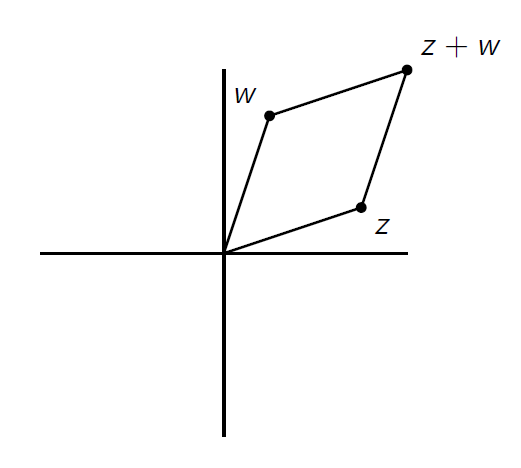
\includegraphics[scale=0.7]{Complex addition.png}
\end{figure}\end{center}
\underline{Multiplication}:
\begin{equation}
    \begin{aligned}
        z&=a+bi\neq0\\
        &=r \cos\theta+r \sin\theta i\\
        &=r (\cos\theta+i\sin\theta)\\
        |z|^2&=a^2+b^2=r^2
    \end{aligned}
    \nonumber
\end{equation}
\begin{equation}
    \begin{aligned}
        z=&r (\cos\theta+i\sin\theta)\\
        w=&s (\cos\phi+i\sin\phi)\\
        zw=&rs[\cos\theta\cos\phi-\sin\theta\sin\phi+i(\cos\theta\sin\phi+\cos\phi\sin\theta)]\\
        =&rs[cos(\theta+\phi)+i\sin(\theta+\phi)]\\
        =&|z||w|[cos(\theta+\phi)+i\sin(\theta+\phi)]
    \end{aligned}
    \nonumber
\end{equation}
\begin{center}\begin{figure}[htbp]
    \centering
    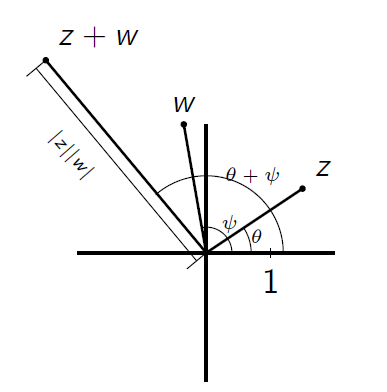
\includegraphics[scale=0.8]{Complex multiplication.png}
\end{figure}\end{center}
We will write,
\begin{equation}
    \begin{aligned}
        &\cos \theta+i\sin\theta=e^{i\theta}\\
        &e^{i\theta}e^{i\phi}=e^{i(\theta+\phi)}\\
        &z=|z|e^{i\theta}
    \end{aligned}
    \nonumber
\end{equation}
\subsection{Theorem 2.1.1: $f(x)=a_0+a_1x+...+a_nx^n$ with coefficients $a_0,a_1,...,a_n\in\mathbb{C}$. Then $f$ has a \underline{root} in $\mathbb{C}$: $\exists \alpha\in\mathbb{C}$ s.t. $f(\alpha)=0$}
\begin{theorem}[Theorem 2.1.1]
Supose a nonconstant polynomial $f(x)=a_0+a_1x+...+a_nx^n$ with coefficients $a_0,a_1,...,a_n\in\mathbb{C}$. Then $f$ has a \underline{root} in $\mathbb{C}$: $\exists \alpha\in\mathbb{C}$ s.t. $f(\alpha)=0$.
\end{theorem}
\subsubsection{Corollary 2.1.2: $f(x)=a_n\prod_{i=1}^n(x-k_i)=a_n(x-k_1)(x-k_2)...(x-k_n)$, where $k_1,k_2,...,k_n$ are roots of $f(x)$}
\begin{corollary}[Corollary 2.1.2]
    Every nonconstant polynomial with coefficients $a_0,a_1,...,a_n\in\mathbb{C}$ can be factored as $f(x)=a_n\prod_{i=1}^n(x-k_i)=a_n(x-k_1)(x-k_2)...(x-k_n)$, where $k_1,k_2,...,k_n$ are roots of $f(x)$.
\end{corollary}
\subsubsection{Corollary 2.1.3: $a_i\in \mathbb{R}$, $f$ can be expresses as a product of linear and quadratic polynomials}
\begin{corollary}[Corollary 2.1.3]
    If $f (x) = a_0 + a_1x + ... + a_nx^n$ is a nonconstant
    polynomial $a_0, a_1, ..., a_n \in \mathbb{R}, a_n \neq 0$.
    Then $f$ can be expresses as a product of linear and quadratic polynomials.
\end{corollary}
这里$a_0, a_1, ..., a_n$是实数!
\begin{proof}
\quad\\
(1)Obviously, the corollary holds at $n=1$ and $n=2$.\\
(2)Suppose the corollary holds for all situations that $n<k$.\\
When $n=k$, $f (x) = a_0 + a_1x + ... + a_kx^k, a_k\neq 0$.\\
By F.T.A., $f$ has a root $\alpha$ in $\mathbb{C}$.\\
If $\alpha\in\mathbb{R}$, long division $f(x)=q(x)(x-\alpha)$. $q$ has real coefficients, $\textit{degree of }q=k-1$. Since the corollary holds at $n=k-1$, $q(x)$ is a product of linear and quadratics. Then, the corollary also holds at $n=k$.\\
If $\alpha\notin\mathbb{R}$
\begin{equation}
    \begin{aligned}
        &0=f(\alpha)=a_0+a_1\alpha+...+a_k\alpha^k\\
        &0=\overline{f(\alpha)}={a_0}+{a_1}\bar{\alpha}+...+{a_n}\bar{\alpha}^n=f(\bar{\alpha})
    \end{aligned}
    \nonumber
\end{equation}
Since $\bar{\alpha}\neq\alpha$, $(x-\alpha)(x-\bar{\alpha})|f$.\\
$(x-\alpha)(x-\bar{\alpha})=x^2-(\alpha+\bar{\alpha})x+|\alpha|^2$ is a polynomial with coefficients in $\mathbb{R}$. So $f(x)=q(x)(x^2-(\alpha+\bar{\alpha})x+|\alpha|^2)$, $q$ has real coefficients with degree $k-2$. The corollary also holds at $n=k-2$, $q(x)$ is a product of linear and quadratics. Then, the corollary also holds at $n=k$.\\
\end{proof}

\section{Field $(\mathbb{F}, +, \cdot)$ (close, associative, commutative, distributive(M over A), identity $\&$ inverse(M,A))}
\textbf{\underline{Definition}}: A \underline{field} is a nonempty set $\mathbb{F}$ with two operations:\\
1. \underline{addition}, written $a+b, \forall a,b\in\mathbb{F}$; \\
2. \underline{multiplication}, written $a\cdot b=ab, \forall a,b\in\mathbb{F}$.\\
such that:\\
(i) \textit{addition} and \textit{multiplication} are \underline{associative} and \underline{commutative}\\
(ii) \textit{multiplication} \underline{distributes} over \textit{addition}: $a(b+c)=ab+ac, \forall a,b,c\in\mathbb{F}$\\
(iii) $\exists$ an \underline{additive identity} $0\in \mathbb{F}$ s.t. $0+a=a, \forall a\in \mathbb{F}$.\\
(iv)$\forall a\in\mathbb{F}$, $\exists$ an \underline{additive inverse} $-a$ s.t. $a+(-a)=0, \forall a\in\mathbb{F}$.\\
(v) $\exists$ a \underline{multiplicative identity}: $1\in\mathbb{F}$ s.t. $1a=a, \forall a\in\mathbb{F}, 1\neq 0$.\\
(vi) $\forall a\in\mathbb{F}, a\neq 0$, $a$ has a \underline{multiplicative inverse} $a^{-1}=\frac{1}{a}\in\mathbb{F}: a\cdot\frac{1}{a}=1$.
\begin{proposition}[Proposition 2.2.2]
$\mathbb{F}$ a field, $a,b\in\mathbb{F}$, then
\end{proposition}
(i) If $a + b = b$ then $a = 0$\\
(ii) If $ab = b$ and $b \neq 0$, then $a = 1$\\
(iii) $0a = 0$\\
(iv) If $ a + b = 0$, then $b = -a$\\
(v) If $a \neq 0$ and $ab = 1$, then $b = a^{-1}$\\
\begin{example}
$\mathbb{Z}_4$ is not a field. Because $[2]_4$ doesn't have \underline{multiplicative inverse} in $\mathbb{Z}_4$.
\end{example}

\subsection{Subfield $(\mathbb{K},+,\cdot)$: $\mathbb{K}\subseteq \mathbb{F}$, closed under $+,\cdot$ and inverse}
\textbf{\underline{Definition}}:Suppose $\mathbb{F}$ is a field and $\mathbb{K}\subseteq \mathbb{F}$ s.t.
\begin{equation}
    \begin{aligned}
        &0,1\in\mathbb{K}\\
        &\forall a,b\in\mathbb{K}, a+b,ab,-a,a^{-1}(\textit{if }a\neq0)\in\mathbb{K}
    \end{aligned}
    \nonumber
\end{equation}
We call $\mathbb{K}$ a \underline{subfield} of $\mathbb{F}$.
\begin{example}
$\mathbb{Q}\subseteq\mathbb{R},\mathbb{R}\subseteq\mathbb{C},\mathbb{Q}\subseteq\mathbb{C}$
\end{example}
\begin{example}
    $\mathbb{K}\subseteq \mathbb{Z}_p$ a subfield $\Rightarrow$ $\mathbb{K}=\mathbb{Z}_p$. Prove by induction.
\end{example}

\subsubsection{Proposition 2.2.3: Subfield 继承 operations 自成一field}
\begin{proposition}[Proposition 2.2.3]
    Suppose $\mathbb{K}\subset \mathbb{F}$ is a subfield of a field $\mathbb{F}$
    Then the operations of $\mathbb{F}$ make $\mathbb{K}$ into a field.
\end{proposition}
$\Rightarrow$We can prove a set is a field by proving it is a subfield of a known field.


\section{Polynomials}
Let $\mathbb{F}$ be any field. A polynomial over $\mathbb{F}$ in variable $x$ is a formal sum:
\begin{equation}
    \begin{aligned}
        a_0+a_1x+a_2x^2+...+a_nx^n=\sum_{i=0}^na_ix^i
    \end{aligned}
    \nonumber
\end{equation}
where $n\geq 0$ is an integer, $a_1,a_1,...,a_n\in\mathbb{F}$.\\
Polynomial is a squence $\{a_k\}_{k=0}^{\infty}$ with $a_m=0,\forall m>n$.
\subsection{$\mathbb{F}[x]$: Polynomial ring 在一个field上形成的所有多项式(方程)的集合}
Let $\mathbb{F}[x]$ denote the set of all polynomials with coefficients in the field $\mathbb{F}$.
\begin{equation}
    \begin{aligned}
        \mathbb{F}[x]=\{\sum_{i=0}^na_ix^i|n\geq0,n\in\mathbb{Z}, a_0,...,a_n\in\mathbb{F}\}
    \end{aligned}
    \nonumber
\end{equation}
We call the $\mathbb{F}[x]$ \textit{polynomial ring} over the field $\mathbb{F}$.
\begin{equation}
    \begin{aligned}
        &f=\sum_{i=0}^na_ix^i, g=\sum_{j=0}^na_jx^j \in\mathbb{F}[x]\\
        &f+g=\sum_{i=0}^n(a_i+b_i)x^i\in\mathbb{F}[x]\\
        &fg(\sum_{i=0}^na_ix^i)(\sum_{j=0}^na_jx^j)=\sum_{i=0}^{2n}(\sum_{j=0}^ia_jb_{i-j})x^i
    \end{aligned}
    \nonumber
\end{equation}

\subsubsection{Proposition 2.3.2: Polynomial ring (close, associative, commutative, distributive(M over A), identity(M,A), inverse(only A))}
\begin{proposition}[Proposition 2.3.2]
Suppose $\mathbb{F}$ is any field. Then,
\end{proposition}
(i) Addition and multiplication are commutative $\&$ associative operations on $\mathbb{F}[x]$\\
(ii) Multiplication distributes over addition\\
(iii) $0 \in \mathbb{F}$, is additive identity in $F[x]: \forall f \in \mathbb{F}[x], f + 0 = 0$\\
(iv) $\forall f \in \mathbb{F}[x], f = (-1)f$ is the additive inverse: $f + (-1)f = 0$.\\
(v) $1 \in \mathbb{F}$, is the multiplicative identity in $\mathbb{F}[x]:\ 1f = f,\  \forall f \in \mathbb{F}[x]$

\subsection{Degree of a Polynomial: $deg(f)$}
$f=\sum_{i=0}^na_ix^i$, $deg(f)=$ degree of $f$ is,
\begin{equation}
    \begin{aligned}
        deg(f)=\left\{\begin{matrix}
            0& \textit{if $f$ is constant, $f\neq0$}\\
            n& \textit{if $a_n\neq0$ in above ($a_n=$ leading coefficent)}\\
            -\infty& \textit{if } f=0
        \end{matrix}\right.
    \end{aligned}
    \nonumber
\end{equation}
Define $-\infty+ a = a + (-\infty) = -\infty\ \forall a \in \mathbb{Z} \cup \{-\infty\}$
\subsubsection{Lemma 2.3.3: $deg(fg)=deg(f)+deg(g)
,\ deg(f+g)\leq\max\{deg(f),deg(g)\}$}
\begin{lemma}[Lemma 2.3.3]
    For any field $\mathbb{F}$ and $f$ , $g \in \mathbb{F}[x]$,
    \begin{equation}
        \begin{aligned}
            &deg(fg)=deg(f)+deg(g)\\
            &deg(f+g)\leq\max\{deg(f),deg(g)\}
        \end{aligned}
        \nonumber
    \end{equation}
\end{lemma}


\subsection{Corollary 2.3.5: Unit(invertible) in $\mathbb{F}[x]$: constant$\neq 0$ iff $deg(f)=0$}
\begin{corollary}[Corollary 2.3.5]
    For any field $\mathbb{F}$ and $f \in \mathbb{F}[x]$, Then $f$ is a $\underline{unit}$(i.e. invertible) in $\mathbb{F}[x]$ iff $deg(f)=0$.
\end{corollary}
\begin{proof}
\quad\\
Obviously, $deg(f)=0\Rightarrow\ f$ is a unit.\\
Suppose $f$ is a unit, i.e. $\exists g\in\mathbb{F}[x]$ s.t. $fg=1$.\\
$0=deg(fg)=deg(f)+deg(g)\Rightarrow deg(f),deg(g)\geq0\Rightarrow deg(f)=0,deg(g)=0.$
\end{proof}
\subsection{\underline{Irreducible} Polynomials: “无法分解为两个$degree\geq1$的多项式积”的多项式: 至少一个是constant (i.e. $degree=0$)}
A nonconstant polynomial $f$ is \underline{irreducible} if $f=uv,\ u,v\in\mathbb{F}[x]$, then either $u$ or $v$ is a unit(i.e., constant$\neq0$)


\subsection{Theorem 2.3.6:nonconstant polynomials可以被唯一地分解}
\begin{theorem}[Theorem 2.3.6]
Suppose $\mathbb{F}$ is a field and $f\in\mathbb{F}[x]$ is any nonconstant. Then $f = ap_1p_2\dots p_k$ where $a \in \mathbb{F},\ p_1,\dots p_k \in \mathbb{F}[x]$ are irreducible \underline{monic} polynomials (monic = i.e. leading coeff. 1). If $f = bq_1q_2\dots q_r$ with $b \in \mathbb{F}$ and
$q_1,q_2,\dots ,q_r \in \mathbb{F}[x]$ monic irreducible, then $a = b, k = r$, and after reindexing $p_i = q_i,\ \forall i$
\end{theorem}


\begin{lemma}[Lemma 2.3.7]
    Suppose $\mathbb{F}$ is a field and $f\in\mathbb{F}[x]$ is nonconstant monic polynomial. Then $f = p_1p_2\dots p_k$ where each $p_i$ is monic irreducible.
\end{lemma}
\begin{proof}
\quad\\
Prove it by induction. When $deg(f)=1,\ f=uv,\ u,v\in\mathbb{F}[x]$, $deg(f)=deg(u)+deg(v)\Rightarrow$ one of these is 0.\\
Suppose the lemma holds for all degree$<n$. When $deg(f)=n$,\\
Either $f$ is irreducible, done.\\
Suppose $f = uv$ with/ $deg(u), deg(v)\geq 1$\\
$\Rightarrow deg(u),deg(v)<n\Rightarrow u=p_1p_2\dots p_k, v=q_1q_2\dots q_j$
So, $f = p_1p_2\dots p_kq_1q_2\dots q_j$.
\end{proof}
\begin{example}
$x^2-1\in\mathbb{Q}[x]$ reducible\\
$x-1,x+1\in\mathbb{Q}[x]$ irreducible\\
$x^2+1\in\mathbb{Q}[x]$ irreducible\\
$x^2+1\in\mathbb{C}[x]$ reducible\\
$x^2-1=x^2+1=[1]x^2+[1]\in\mathbb{Z}_2[x]$ reducible\\
\end{example}

\subsection{Divisibility of Polynomials}
$f,g\in\mathbb{F}[x], f\neq0$, $f$ \underline{divides} $g$, $f|g$ means $\exists u\in\mathbb{F}[x]$ s.t. $g=fu$.
\begin{proposition}[Proposition 2.3.8]
    $f , h, g \in \mathbb{F}[x]$, then
\end{proposition}
(i) If $f \neq 0, f |0$\\
(ii) If $f |1$, $f$ is nonzero constant\\
(iii) If $f |g$ and $g|f$ , then $f = cg$ for some $c \in \mathbb{F}$\\
(iv) If $f |g$ and $g|h$, then $f |h$\\
(v) If $f|g$ and $f|h$, then $f|(ug + vh)$ for all $u, v \in \mathbb{F}[x]$.\\


\subsubsection{Greatest common divisor of $f$ and $g$: is not unique, we denote monic Greatest common divisor as $gcd(f,g)$}
If $f, g \in \mathbb{F}[x]$ are nonzero polynomials, a \underline{greatest common divisor} of $f$ and $g$ is a polynomial $h \in \mathbb{F}[x]$ such that\\
(i) $h|f$ and $h|g$, and\\
(ii) if $k\in\mathbb{F}[x]$ and $k|f$ and $k|g$, then $k|h$.\\
the $gcd$ is not unique, but the monic $gcd$ is unique. We call it \textbf{the monic greatest common divisor}, denote it $gcd(f,g)$.
\begin{example}
\begin{equation}
    \begin{aligned}
        &x^2 - 1, x^2 - 2x + 1 \in \mathbb{Q}[x]\\
        &(x - 1)(x + 1), (x - 1)^2 \in \mathbb{Q}[x]\\
        &x -1 = gcd(x^2 - 1, x^2 - 2x + 1)
    \end{aligned}
    \nonumber
\end{equation}
\end{example}

\subsubsection{Proposition 2.3.9: Euclidean Algorithm of polynomials}
\begin{proposition}[Proposition 2.3.9]
    Given $f, g \in \mathbb{F}[x]$, $g \neq 0$, then $\exists q, r \in \mathbb{F}[x]$ s.t.
    $deg(r ) < deg(g)$
    and $f = qg + r$
\end{proposition}
\begin{example}
\begin{equation}
    \begin{aligned}
        &f = 3x^3 - 5x^2 - 3x + 5, g = x^3 − 2x^2 + 1 \in \mathbb{Q}[x]\\
        &f=3g+x^2-3x+2
    \end{aligned}
    \nonumber
\end{equation}
\end{example}

\subsubsection{Proposition 2.3.10: $gcd(f,g)$ 是degree最小的f,g的线性组合}
\begin{proposition}[Proposition 2.3.10]
    Any 2 nonzero polynomials $f , g \in \mathbb{F}[x]$ have
    a gcd in $\mathbb{F}[x]$. In fact among all polynomials
    in the set
    $M = \{uf + vg|u, v \in \mathbb{F}[x]\}$
    any nonconstant of minimal degree are gcds.
\end{proposition}
\begin{proof}
\quad\\
$h\in M$, $deg(h)=d$ minimal. Let $k|f$ and $k|g$ $\Rightarrow$ $k|uf+vg,\ \forall u,v\Rightarrow k|h$.\\
Suppose $h'\in M$ is any nonzero element. $deg(h')\geq deg(h)\Rightarrow\ \exists q,r\in\mathbb{F},deg(r)<deg(h)\ h'=qh+r$. $r=h'-qh\in M$. Since $deg(h)=d$ is nonconstant minimal degree, $r=0\Rightarrow h'=qh$. So $\exists q_1,q_2\in\mathbb{F}[x],\ 1f+0g=q_1h, 0f+1g=q_2h$ $\Rightarrow h|g,h|f$.
\end{proof}
\begin{example}
    \begin{equation}
        \begin{aligned}
            &f = 3x^3 - 5x^2 - 3x + 5, g = x^3 − 2x^2 + 1 \in \mathbb{Q}[x]\\
            &f=3g+x^2-3x+2\\
            &g=(x+1)(x^2-3x+2)+x-1\\
            &x^2-3x+2=(x-2)(x-1)\\
            &\Rightarrow gcd(f,g)=x-1\\
            &x-1=g-(x+1)(x^2-3x+2)=g-(x+1)(f-3g)=(3x+4)g-(x+1)f
        \end{aligned}
        \nonumber
    \end{equation}
\end{example}

\begin{example}
    Find a greatest common divisor of $f=x^3-x^2-x+1$ and $g=x^2-3x+2$ in $\mathbb{Q}[x]$, and express it in form $uf+vg,\ u,v\in\mathbb{Q}[x]$.
\end{example}
\begin{equation}
    \begin{aligned}
        &f=(x+2)g+3x-3\\
        &g=\frac{1}{3}(x-2)(3x-3)\\
        &gcd(f,g)=3x-3\\
        &3x-3=f-(x+2)g
    \end{aligned}
    \nonumber
\end{equation}


\subsubsection{Proposition 2.3.12: $gcd(f,g)=1, f|gh\Rightarrow f|h$}
\begin{proposition}[Proposition 2.3.12]
If $f,g,h\in\mathbb{F}[x]$, $gcd(f,g)=1$, and $f|gh$, then $f|h$.
\end{proposition}

\subsubsection{Corollary 2.3.13: irreducible $f$, $f|gh$ $\Rightarrow f|g$ or $f|h$}
\begin{corollary}[Corollary 2.3.13]
If $f\in\mathbb{F}[x]$ is irreducible, and $f|gh$, then $f|g$ or $f|h$.
\end{corollary}
Since $f$ is irreducible, we have two possible situations:\\
1. $gcd(f,g)=f$, i.e. $f|g$ done.\\
2. $gcd(f,g)=1$, then according to Prop 2.3.12, we can know $f|h$.\\


\subsection{Roots}
\underline{Root}:$\alpha\in\mathbb{F}$ is a root of $f$ if $f(\alpha)=0$.

\subsubsection{Corollary 2.3.16(of Euclidean Algorithm): $f$ 可被分为 $(x-\alpha)q+f(\alpha)$i.e. if $\alpha$ is a root, then $(x-\alpha)|f$}
\begin{corollary}[Corollary 2.3.16(of Euclidean Algorithm)]
$\forall f\in\mathbb{F}[x]$ and $\alpha\in\mathbb{F}$, there exists a polynomial $q\in\mathbb{F}[x]$ s.t. $f=(x-\alpha)q+f(\alpha)$. In particular , if $\alpha$ is a root, then $(x-\alpha)|f$.
\end{corollary}

\subsection{Multiplicity}
If $\alpha$ is a root of $f$ , say its \textit{multiplicity} is $m$, if $x-\alpha$ appears $m$ times in irreducible factorization.
\subsubsection{$\textit{Sum of multiplicity}\leq deg(f)$}
\begin{proposition}[Proposition 2.3.17]
Given a nonconstant polynomial $f\in\mathbb{F}[x]$, the number of roots of $f$, counted with multiplicity, is at most $deg(f)$.
\end{proposition}

\subsection{Roots in a filed may not in its subfield}
Note if $\mathbb{F}\subset \mathbb{K}$, then $\mathbb{F}[x]\subset\mathbb{K}$. $f\in\mathbb{F}[x]$ may have no roots in $\mathbb{F}$, but could have roots in $\mathbb{K}$
\begin{example}
    $x^n-1\in\mathbb{Q}[x]$ has a root in $\mathbb{Q}$: 1; has 2 roots if $n$ even: $\pm 1$\\
    $\underline{roots\ in\ \mathbb{C}}:\zeta_n=e^{\frac{2\pi i}{n}}$, then $\zeta_n^n=e^{2\pi i}=1$; $(\zeta_n^k)^n=e^{2\pi ki}=1$ So, the roots: $\{e^{\frac{2\pi ki}{n}}|k=0,...,n-1\}$\\
    The roots of $x^n-d$: $\{e^{\frac{2\pi ki}{n}}\sqrt{d}|k=0,...,n-1\}$\\
\end{example}

\section{Linear Algebra}
\subsection{ Vector Space $(V,+,\times)$ (over a field $\mathbb{F}$)}
A \underline{vector space} over a field $\mathbb{F}$ is a
set $V$ w/ an operation \underline{addition} $+ : V \times V \rightarrow V$ and
an operation \underline{scalar multiplication} $\mathbb{F} \times V \rightarrow V$\\
(1) Addition is associative $\&$ commutative\\
(2) $\exists 0\in V$, additive identity: $0 + v = v \forall v \in V$\\
(3) $1v = v \forall v \in V$(where $1 \in \mathbb{F}$ is multi. id. in $\mathbb{F}$ )\\
(4) $\forall \alpha,\beta\in\mathbb{F},\ v\in V,\ \alpha(\beta v)=(\alpha\beta)v$\\
(5) $\forall v\in V,\ (-1)v=-v$ we have $v+(-v)=0$\\
(6) $\forall \alpha\in\mathbb{F},\ v,u\in V,\ \alpha(v+u)=\alpha v+\alpha u$\\
(7) $\forall \alpha,\beta\in\mathbb{F},\ v\in V,\ (\alpha+\beta)v=\alpha v+\beta v$

\subsubsection{A field is a vector space over its subfield}
\begin{example}
$\mathbb{K}\subset\mathbb{F}$ is a subfield of a field $\mathbb{F}$. Then $\mathbb{F}$ is a vector space over $\mathbb{K}$. (Since $\mathbb{F}\subset \mathbb{F}[x]$, then $\mathbb{F}[x]$ is a vector space over $\mathbb{F}$.)
\end{example}
\subsubsection{ Vector subspace}
Suppose that $V$ is a vector space over $\mathbb{F}$. A \underline{vector subspace} or just \underline{subspace} is a nonempty subset $W\subset V$ closed under addition and scalar multiplication. i.e. $v+w\in W,\ av\in W,\ \forall v,w\in W,\ a\in \mathbb{F}$.\\
\begin{example}
$\mathbb{K}\subset \mathbb{L}\subset \mathbb{F}$, then $\mathbb{L}$ is a subspace of $\mathbb{F}$ over $\mathbb{K}$.
\end{example}
\subsection{Linear independent, Linear combination}
\subsection{span V, basis, dimension, Proposition 2.4.10}
A set of elements $v_1,...,v_n\in V$ is said to \textbf{span} $V$ if every vector $v\in V$ can be expressed as a linear combination of $v_1,...,v_n$. If $v_1,...,v_n$ spans and is linearly independent, then we call the set a \textbf{\textit{basis}} for $V$.
\begin{proposition}[Proposition 2.4.10.]
    Suppose $V$ is a vector space over a field $\mathbb{F}$ having a basis $\{v_1,...,v_n\}$ with $n \geq 1$.
\end{proposition}
(i) For all $v \in V$ , $v = a_1 v_1 + ... + a_n v_n$ for exactly one $(a_1,...,a_n)\in \mathbb{F}^n$.\\
(ii) If $w_1,...,w_n$ span $V$ , then they are linearly independent.\\
(iii)If $w_1,...,w_n$ are linearly independent, then they span $V$.\\
If a vector space $V$ over $\mathbb{F}$ has a basis with $n$ vectors, then $V$ is said to be n-dimensional (over $\mathbb{F}$) or is said to have \textbf{dimension} $n$.
\subsubsection{Standard basis vectors}
\begin{equation}
    \begin{aligned}
        e_1=(1,0,...,0),e_2=(0,1,0,...,0),...,e_n=(0,0,...,0,1)\in \mathbb{F}^n
    \end{aligned}
    \nonumber
\end{equation}
are a basis for $\mathbb{F}^n$ called the \textbf{standard basis vectors}.
\subsection{Linear transformation}
Given two vector spaces $V$ and $W$ over $\mathbb{F}$ a \textbf{linear transformation} is a function $T : V \rightarrow	 W$ such that
for all $a \in \mathbb{F}$ and $v,w \in V$ , we have
\begin{equation}
    \begin{aligned}
        T(av)=aT(v)\ and\ T(v+w)=T(v)+T(w)
    \end{aligned}
    \nonumber
\end{equation}
\begin{proposition}[Proposition 2.4.15.]
    If $V$ and $W$ are vector spaces and $v_1,...,v_n$ is a basis for $V$ then any function
    from $\{v_1,...,v_n\}\rightarrow W$ extends \textit{uniquely} to a linear transformation $V \rightarrow W$.
\end{proposition}
Any $v\in V$, $\exists (a_1,...,a_n)$ s.t. $v=a_1 v_1+...+a_n v_n$. Then $T(v)=T(a_1 v_1+...+a_n v_n)=a_1T(v_1)+...+a_nT(v_n)$\\
\subsubsection{Corollary 2.4.16: 一个线性变换对应一个矩阵 \textit{bijection} $\mathcal{L} (V,M)\rightarrow M_{m\times n}(\mathbb{F})$}
\begin{corollary}[Corollary 2.4.16.]
    If $v_1,...,v_n$ is a basis for a vector space $V$ and $w_1,...,w_n$ is a basis for a vector space $W$ (both over $\mathbb{F}$), then any linear transformation $T : V \rightarrow W$ determines (and is determined by) the $m\times n$ matrix:
    \begin{equation}
        \begin{aligned}
            A=A(T)=\begin{bmatrix}
                A_{11}&	A_{12}&... &A_{1n}\\
                A_{21}&	A_{22}&... &A_{2n}\\
                \vdots&	\vdots&... &\vdots\\
                A_{m1}&	A_{m2}&... &A_{mn}
            \end{bmatrix}
        \end{aligned}
        \nonumber
    \end{equation}
\end{corollary}
\begin{equation}
    \begin{aligned}
        &\begin{bmatrix}
            w_1&\cdots	&w_m
        \end{bmatrix}^T=A
        &\begin{bmatrix}
                v_1&\cdots	&v_n
        \end{bmatrix}^T
    \end{aligned}
    \nonumber
\end{equation}
$\mathcal{L} (V,M)$ denotes the set of all linear transformations from $V$ to $W$; $M_{m\times n}(\mathbb{F})$ the set of $m\times n$ matrix with entries in $\mathbb{F}$. $T\rightarrow A(T)$ defines a \textit{bijection} $\mathcal{L} (V,M)\rightarrow M_{m\times n}(\mathbb{F})$. \textbf{$A(T)$ represents the linear transformation $T$}.

\subsubsection{Proposition 2.4.19: 线性变换矩阵相乘仍为线性变换矩阵}
\begin{proposition}[Proposition 2.4.19]
    Suppose that $V$ , $W$, and $U$ are vector spaces over $\mathbb{F}$, with fixed chosen bases. If
    $T : V \rightarrow W$ and $S : W \rightarrow U$ are linear transformations represented by matrices $A = A(T)$ and $B = B(S)$,
    then $ST = S \circ T : V \rightarrow U$ is a linear transformation represented by the matrix $BA = B(S)A(T)$.
\end{proposition}

\subsection{GL(V): invertible(bijective) linear transformations $V \rightarrow	V$}
Given a vector space $V$ over $F$, we let $GL(V ) \subset \mathcal{L}(V , V )$ denote the subset of \textbf{invertible linear transformations}.
\begin{equation}
    \begin{aligned}
        GL(V)=\{T\in \mathcal{L}(V , V )| T \textit{ is a bijection}\}=\mathcal{L}(V , V )\cap Sym(V)
    \end{aligned}
    \nonumber
\end{equation}

\section{Euclidean geometry basics}
\subsection{ Euclidean distance, inner product}
\textbf{Euclidean distance} on $\mathbb{R}^n$:
\begin{equation}
    \begin{aligned}
        |x-y|=\sqrt{(x_1-y_1)^2+...+(x_n-y_n)^2}
    \end{aligned}
    \nonumber
\end{equation}
\textbf{Euclidean inner product}:
\begin{equation}
    \begin{aligned}
        x\cdot y=x_1y_1+\cdots +x_ny_n=x^Ty
    \end{aligned}
    \nonumber
\end{equation}
\subsection{Isometry of $\mathbb{R}^n$: a bijection $\mathbb{R}^n \rightarrow \mathbb{R}^n$ preserves distance}
An \textbf{isometry} of $\mathbb{R}^n$ is a bijection $\varPhi :\mathbb{R}^n \rightarrow \mathbb{R}^n$ that preserves distance, which means,
\begin{equation}
    \begin{aligned}
        |\varPhi(x)-\varPhi(y)|=|x-y|,\ \forall x,y\in \mathbb{R}^n
    \end{aligned}
    \nonumber
\end{equation}
\subsubsection{$Isom(\mathbb{R}^n)$: set of all isometries of $\mathbb{R}^n$}
We use $Isom(\mathbb{R}^n)$ denotes the set of all isometries of $\mathbb{R}^n$,
\begin{equation}
    \begin{aligned}
        Isom(\mathbb{R}^n)=\{\varPhi:\mathbb{R}^n \rightarrow \mathbb{R}^n | |\varPhi(x)-\varPhi(y)|=|x-y|,\ \forall x,y\in \mathbb{R}^n\}
    \end{aligned}
    \nonumber
\end{equation}

\subsubsection{$Isom(\mathbb{R}^n)$ is closed under $\circ$ and inverse}
\begin{proposition}
$\varPhi, \varPsi \in Isom(\mathbb{R}^n)$, then $\varPhi\circ\varPsi, \varPhi^{-1}\in Isom(\mathbb{R}^n)$
\end{proposition}
\begin{proof}
\quad\\
Since $\varPhi,\varPsi$ are bijections, so is $\varPhi\circ\varPsi$. Moreover,\\
\begin{equation}
    \begin{aligned}
        &|\varPhi\circ\varPsi(x)-\varPhi\circ\varPsi(y)|=|\varPhi(\varPsi(x))-\varPhi(\varPsi(y))|=|\varPsi(x)-\varPsi(y)|=|x-y|\\
    \end{aligned}
    \nonumber
\end{equation}
Since $id\in Isom (\mathbb{R}^n)$,
\begin{equation}
    \begin{aligned}
        |x-y|=|id(x)-id(y)|=|\varPhi\circ\varPhi^{-1}(x)-\varPhi\circ\varPhi^{-1}(y)|=|\varPhi^{-1}(x)-\varPhi^{-1}(y)|
    \end{aligned}
    \nonumber
\end{equation}
\end{proof}

\subsection{$A\in GL(n,\mathbb{R})$, $T_A(v)=Av$: $A^tA=I \Leftrightarrow T_A\in Isom(\mathbb{R}^n)$}
There is a matrix $A\in GL(n,\mathbb{R})$ i.e. a \textit{invertible linear transofrmations} $T_A: \mathbb{R}^n \rightarrow \mathbb{R}^n$ is given by $T_A(v)=Av$.
\begin{equation}
    \begin{aligned}
        T_A(v)\cdot T_A(w)=(Av)\cdot(Aw)=(Av)^t(Aw)=v^tA^tAw
    \end{aligned}
    \nonumber
\end{equation}
\begin{equation}
    \begin{aligned}
        A^tA=I\Leftrightarrow T_A(v)\cdot T_A(w)=v\cdot w\Leftrightarrow_{(HW4)}\ T_A\in Isom(\mathbb{R}^n)
    \end{aligned}
    \nonumber
\end{equation}
\subsection{ Linear isometries i.e. orthogonal group $O(n)=\{A\in GL(n,\mathbb{R})|A^tA=I \}$}
We define the all isometries in \textit{invertible linear transofrmations} $\mathbb{R}^n \rightarrow \mathbb{R}^n$ as \textbf{orthogonal group}
\begin{equation}
    \begin{aligned}
        O(n)=\{A\in GL(n,\mathbb{R})|A^tA=I \}\subset GL(n,\mathbb{R})
    \end{aligned}
    \nonumber
\end{equation}

\subsubsection{Special orthogonal group $SO(n)=\{A\in O(n) | det(A)=1\}$: orthogonal group with $det(A)=1$}
$O(n)$ are the matrices representing linear isometries of $\mathbb{R}^n$.
$1=det(I)=det(A^tA)=det(A^t)det(A)=det(A)^2 \Rightarrow	det(A)=1$ or $det(A)=-1$. We use \textbf{special orthogonal group} represents $A$ with $det(A)=1$,
\begin{equation}
    \begin{aligned}
        SO(n)=\{A\in O(n) | det(A)=1\}
    \end{aligned}
    \nonumber
\end{equation}

\subsection{translation: $\tau_v(x)=x+v$}
Define a \textit{translation} by $v\in \mathbb{R}^n$,
\begin{equation}
    \begin{aligned}
        \tau_v:\mathbb{R}^n \rightarrow \mathbb{R}^n,\ \tau_v(x)=x+v
    \end{aligned}
    \nonumber
\end{equation}
\subsubsection{translation is an isometry}
\begin{note}[Exercise 2.5.3]
$\forall v\in \mathbb{R}^n, \tau_v$ is an isometry.
\end{note}
\begin{proof}
$|\tau_v(x)-\tau_v(y)|=|(x+v)-(y+v)|=|x-y|$
\end{proof}

\subsection{The composition of a translation and an orthogonal transformation is an isometry $\Phi_{A,v}(x)=\tau_v(T_A(x))=Ax+v$}
Since \textit{the composition of isometries is an isometry,} $\forall A\in O(n)$ and $v\in \mathbb{R}^n$, the composition
\begin{equation}
    \begin{aligned}
        \Phi_{A,v}(x)=\tau_v(T_A(x))=Ax+v
    \end{aligned}
    \nonumber
\end{equation}
is an isometry. \textbf{which could account for all isometries}.
\subsubsection{Theorem 2.5.3: All isometries can be represented by a composition of \textit{a translation} and \textit{an orthogonal transformation}, $Isom(\mathbb{R}^n)=\{\Phi_{A,v}|A\in O(n), v\in \mathbb{R}^n \}$}
\begin{theorem}[Theorem 2.5.3]
$Isom(\mathbb{R}^n)=\{\Phi_{A,v}|A\in O(n), v\in \mathbb{R}^n \}$
\end{theorem}



\section{Group}
\subsection{Group $(G, *)$: a set with a binary operation(associative, identity, inverse)}
\subsubsection{Definition}
A \textit{group} is a nonempty set $G$ with a binary operation $*:G \times G \rightarrow G$ s.t.
\begin{enumerate}[(1)]
    \item Binary operation on $G$, $*:G \times G \rightarrow G$
    \item $*$ is \textbf{associative}
    \item $G$ contains an \textbf{identity} element $e$ for $*$: $\exists e\in G$ s.t. $e * g = g * e = g\ \forall g \in G$
    \item Each element $a\in G$ has an \textbf{inverse} $b\in G$ s.t. $a*b=b*a=e$.

A Group is \textbf{abelian} if moreover
    \item $*$ is \textbf{commutative}.
\end{enumerate}

$|G|= $Order of a group $(G,*)$

$(\mathbb{Z},+)$ is a group and $+$ is commutative, we call this kind of groups(statify commutative) \textit{abelian group}.
\begin{example}
If $\mathbb{F}$ is a field, then $(\mathbb{F},+)$ and $(\mathbb{F}^{\times},\cdot)$ are abelian group.
\end{example}
\begin{example}
If $V$ is a vector space over $\mathbb{F}$, then $(V,+)$ abelian group.
\end{example}
As we know a $V$ is a vector space over $\mathbb{F}$ means $V$ is a field whose subfields include $\mathbb{F}$.

\subsubsection{Uniqueness of identity and inverse}
\begin{lemma}
    1. Identity of a group is unique. 2. Inverse of any element in a group is also unique.
\end{lemma}
\begin{proof}
\quad\\
1. Let $e,e'$ be two identities in $G$, then $e*e'=e=e'$.

2. Suppose $b,c$ are both inverse of $a$, then
\begin{equation}
    \begin{aligned}
        b=b*e=b*(a*c)=(b*a)*c=e*c=c
    \end{aligned}
    \nonumber
\end{equation}
\end{proof}



\subsubsection{$(Sym(X),\circ)$ symmetric/permutation group of $X$}
\begin{example}
If $X$ is any nonempty set, permutation group of $X: \{\sigma:X \rightarrow X| \sigma$ is a bijection\}, then
\end{example}
1. $\circ$ is associative;\\
2. $id: X \rightarrow X,\ id(x)=x\ \forall x\in X$ is the idenity;\\
3. $\sigma\in Sym(X), \sigma^{-1}\in Sym(X)$ is the inverse function.\\
\textbf{$(Sym(X),\circ)$ is a group called the symmetric group of $X$}


\subsubsection{Cancelation Laws}
\begin{theorem}
Let $G$ be a group. The left and right cancelation laws hold in $G$:
\begin{enumerate}
    \item $a*x=a*y \Rightarrow x=y$
    \item $x*a=y*a \Rightarrow x=y$
\end{enumerate}
\end{theorem}
\begin{proof}
\quad\\
Let $a*x=a*y$. $\exists a'$ s.t. $a'*a=e$. $a'*(a*x)=a'*(a*y) \Rightarrow (a'*a)*x=(a'*a)*y \Rightarrow	e*x=e*y \Rightarrow	x=y$

Similar for the right cancel law.
\end{proof}

\subsubsection{Unique Solution of Linear Equation}
\begin{theorem}
The linear equation $a*x=b$ and $y*a=b$ has unique solution.
\end{theorem}
\begin{proof}
\quad\\
\begin{enumerate}
    \item Existence: Multiply by $a'$: $a'*(a*x)=a'*b \Rightarrow x=a'*b$ is a solution.
    \item Uniqueness: if $x'$ is another, $a*x=a*x'=b \Rightarrow x=x'$
\end{enumerate}
\end{proof}



\subsection{Subgroup: $H\leq G$}
\begin{definition}
A subset $H\subseteq G$ is a subgroup of $G$ if $H$ is itself a group.
\end{definition}
write $H\leq G$, $H<G$ if $H$ is a subgroup of $(G, *)$. (If $H=G$, $H$ is an improper subgroup. If $H\subsetneq G$, $H$ is an proper subgroup.)

If $H=\{e\}$, then $H$ is a trivial subgroup.

If $H\neq\{e\}$, then $H$ is a nontrivial subgroup.

\begin{theorem}
    A subset $H\subseteq G$ is a subgroup of $G$ if and only if
    \begin{enumerate}
        \item $H$ is closed under $*$. ($\forall\ g,h\in H$, $g*h\in H$)
        \item identity $e\in H$.
        \item Each $a\in H$, the inverse $a'\in H$
    \end{enumerate}
\end{theorem}
\begin{proof}
\quad\\
"$\Rightarrow$": if $H\leq G$ be a subgroup.
\begin{enumerate}
    \item $H$ is a group $\Rightarrow$ $*$ is a binary operation on $H$, $*:H\times H \rightarrow H$ i.e. $H$ is closed under $*$.
    \item Identity of $H$, $e_H$ is also a identity of $G$, due to the uniqueness of identity, $e_H=e_G$.
    \item $a\in H$, $a$'s inverse $a'_H\in H$ is also an inverse in $G$, due to the uniqueness of identity, $a'_H=a'_G$.
\end{enumerate}
"$\Leftarrow$":
\begin{enumerate}
    \item $H$ is closed under $*$ $\Rightarrow	$ $*$ is a binary operation on $H$.
    \item 2,3 fufill the requirement of identity and inverse.
    \item $*$ is operation of group $G$ $\Rightarrow$ $*$ is associative.
    
    Hence $H$ is itself a group.
    \item $H$ is a subeset of $G$, then $H$ is s subgroup of $G$.
\end{enumerate}
\end{proof}


\subsubsection{Proposition 2.6.8: $H<G$, $(H,*)$ is a group: A group's operation with its any subgroup is also a group}
不同的definition.
\begin{proposition}[Proposition 2.6.8]
    If $(G, *)$ is a group, $H \subset G$ is a subgroup, then $(H, *)$ is a group.
\end{proposition}
\begin{example}
    $(G,*)$ is a group, then ${e}<G,\ G<G$.
\end{example}
\begin{example}
$\mathbb{K}\subset \mathbb{F}$ is a subfield, then $\mathbb{K}<\mathbb{F},\ \mathbb{K}^{\times}<\mathbb{F}^{\times}$.
\end{example}
\begin{example}
$W\subset V$ is a vector subspace, $W<V$.
\end{example}
\begin{example}
$1\in S^1\subset \mathbb{C}^{\times}$, $S^1=\{z\in\mathbb{C}| |z|=1\}$. $S^1$ is a subgroup.
\end{example}
\begin{proof}
\quad\\
$S^1=\{e^{i\theta}| \theta\in \mathbb{R}\}$. For any $e^{i\theta}, e^{i\psi}\in S^1$, $e^{i\theta}e^{i\psi}=e^{i(\theta+\psi)}\in S^1, e^{-i\theta}\in S^1$.
\end{proof}
\begin{example}
$Isom(\mathbb{R}^n)<Sym(\mathbb{R}^n)$
\end{example}
\begin{example}
If $\mathbb{F}$ is a field, $Aut(\mathbb{F})=\{\sigma:\mathbb{F}\rightarrow	\mathbb{F}\in Sym(\mathbb{F})| \sigma(a+b)=\sigma(a)+\sigma(b), \sigma(ab)=\sigma(a)\sigma(b)\}<Sym(\mathbb{F})$
\end{example}
\begin{example}
    Dihedral Groups:
\end{example}
保留多边形\\
Let $P_n\subset \mathbb{R}^2$ be a regular $n-gon$
\begin{center}\begin{figure}[htbp]
    \centering
    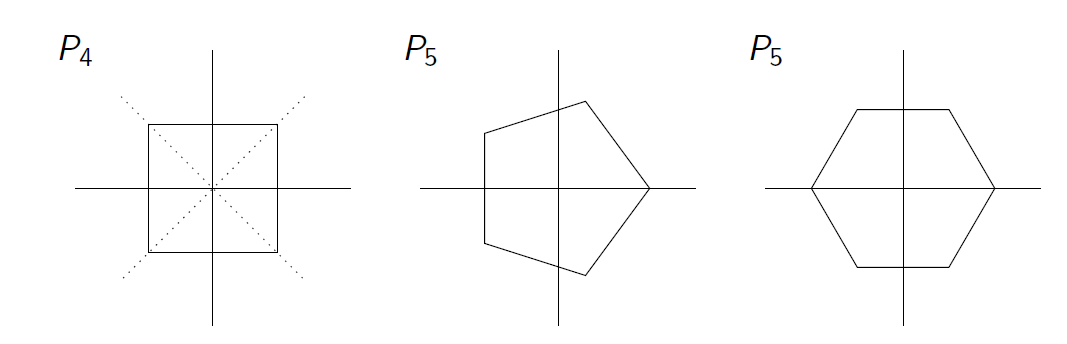
\includegraphics[scale=0.8]{Dihedral Groups.png}
\end{figure}\end{center}
$D_n<Isom(\mathbb{R}^2)$, $D_n=\{\Phi \in Isom(\mathbb{R}^2)|\Phi(P_n)=P_n\}$


\subsection{Some Properties of Group Operation}
\begin{proposition}[Proposition 3.1.1]
    Let $(G,*)$ be a group with identity $e\in G$, then
\end{proposition}
(1) if $g,h\in G$ and either $g*h=h$ or $h*g=h$, then $g=e$\\
(2) if $g,h\in G$ and $g*h=e$ then $g=h^{-1}$ and $h=g^{-1}$

\begin{corollary}[Corollary 3.1.2]
    $e^{-1}=e,\ (g^{-1})^{-1}=g,\ (g*h)^{-1}=h^{-1}*g^{-1}$
\end{corollary}


\subsection{Power of an Element}
We define $g^n$ recursively for $n \geq 0$ by setting $g^0 = e$ and for $n\geq 1$, we set $g^n = g^{n−1} * g$. For $n \leq 0$, we define $g^n = (g^{−1})^{-n}$.
\begin{proposition}[Proposition 3.1.5]
(1) $g^n*g^m=g^{n+m}$; (2) $(g^n)^m=g^{nm}$
\end{proposition}

\subsection{$(G\times H, \circledast)$: \underline{Direct Product} of $G$ and $H$}
$(G,*)$ a group $(H,\star)$ a group. Define an operation on $G\times H$, $\circledast$:\\
$$(h,k)\circledast(h',k')=(h*h',k*k')$$
\subsubsection{Proposition 3.1.7: $(G\times H, \circledast)$ is a group}
\begin{proposition}[Proposition 3.1.7]
$(G\times H, \circledast)$ is a group. The identity is $(e_G,e_H)$, inverse is $(g^{-1},h^{-1})$
\end{proposition}
usually written as
$$(h,k)(h',k')=(hh',kk')$$

\subsection{Subgroups and Cyclic Groups}

\subsubsection{Intersection of Subgroups is a Subgroup}
\begin{proposition}[Proposition 3.2.2]
Let $G$ be a group and suppose $\mathcal{H}$ is any collection of subgroups of $G$. Then $K=\cap_{H\in\mathcal{H}}H<G$ is a subgroup of $G$.
\end{proposition}


\subsubsection{Subgroup Generated by $A$: $\left\langle A\right\rangle$}
We define \textbf{Subgroup Generated by $A$:} $$\left\langle A\right\rangle=\cap_{H\in\mathcal{H}(A)}H$$
where $\mathcal{H}(A)$ is the set of all subgroups of $G$ containing the set $A$:
$$\mathcal{H}(A)=\{H<G|A\subset H \textit{ and }H \textit{ is a subgroup of } G \}$$


\subsubsection{Cyclic Group: group generated by an element}
A group $G$ is \underline{cyclic} if exists $g$ (an element), $\left\langle g\right\rangle=G$.

$g$ is called a \underline{generator} for $G$ in this case.

Easy to prove
$$G=\left\langle g\right\rangle =\{...g^{-2},g^{-1},e,g^1,g^2...\}$$



\subsubsection{Cyclic Subgroup}
If $A$ is a subgroup of $G$, and $A=\left\langle \{a\}\right\rangle=\left\langle a\right\rangle$. Then $A$ is the \underline{cyclic subgroup} generated by $a$: $A=\left\langle a\right\rangle\leq G$

$$\left\langle a\right\rangle =\{...a^{-2},a^{-1},e,a^1,a^2...\}$$


\subsubsection{A Subgroup of a Cyclic Group must be Cyclic}
\begin{theorem}
A subgroup of a cyclic group is cyclic.
\end{theorem}
\begin{proof}
\quad\\
Let $G=\{a^n:n\in \mathbb{Z}\}$ be a cyclic group. Let $H\leq G$ be a subgroup.
\begin{enumerate}
    \item If $H=\{e\}$, then $H$ is cyclic.
    \item If $H\neq \{e\}$, then $a^n\in H$ for some $n>0$. Check $m$ be the minimal among all $n$.
    
    \underline{Claim}: $H=\left\langle a^m\right\rangle$
\end{enumerate}
\end{proof}

\subsubsection{Corollary 3.2.4: $G$ is a cyclic group $\Rightarrow	$ $G$ is abelian}
\begin{corollary}[Corollary 3.2.4]
    If $G$ is a cyclic group (i.e. exits $g\in G$ s.t. $\left\langle g\right\rangle=G$), then $G$ is abelian (i.e. commutative).
\end{corollary}

\subsubsection{Equivalent properties of order of $g$: $|g|=|\left\langle g\right\rangle|<\infty$}
\begin{proposition}[Proposition 3.2.6]
    Let $G$ be a group for $g \in G$, the
    following are equivalent:
\end{proposition}
(i) $|g|<\infty$\\
(ii) $\exists n \neq m$ in $\mathbb{Z}$ so that $g^{n}=g^{m}$\\
(iii) $\exists n \in \mathbb{Z},\ n\neq 0$ so that $g^{n}=e$\\
(iv) $\exists n \in \mathbb{Z}_{+}$so that $g^{n}=e$\\
If $|g|<\infty$, then $|g|=$ smallest $n \in \mathbb{Z}_{+}$so that $g^{n}=e$, and $\langle g\rangle=\left\{e, g, g^{2}, \ldots, g^{n-1}\right\}=\left\{g^{n} \mid n=0, \ldots, n-1\right\}$

\subsubsection{$(\mathbb{Z},+)$ Theorem 3.2.9: $H < \mathbb{Z}$ is a subgroup $\Rightarrow$ $H = \{ 0 \}$ or $H=\left\langle d\right\rangle$; $\left\langle a\right\rangle <\left\langle b\right\rangle$ if and only if $b|a$}
\begin{theorem}[Theorem 3.2.9]
    If $H < \mathbb{Z}$ is a subgroup, then either $H = \{ 0 \}$ , or else $H=\left\langle d\right\rangle$ , where $$d = \min \{ h \in H | h > 0 \}$$
    Consequently, $a \rightarrow \left\langle a\right\rangle$ defines a \textbf{bijection} from $N = \{ 0, 1, 2, . . . \}$ to the set of subgroups of $\mathbb{Z}$. Furthermore,
    for $a,b\in \mathbb{Z}_{+}$, we have $\left\langle a\right\rangle <\left\langle b\right\rangle$ if and only if $b|a$.
\end{theorem}

\subsubsection{$(\mathbb{Z}_n,+)$ Theorem 3.2.10: $H < \mathbb{Z}_n$ is a subgroup $\Rightarrow$ $H=\left\langle [d]\right\rangle$; $\left\langle [d]\right\rangle<\left\langle [d']\right\rangle$ if and only if $d'|d$}
\begin{theorem}[Theorem 3.2.10]
For any $n \geq 2$, if $H <\mathbb{Z}_n$ is a subgroup, then there is a positive divisor $d$ of $n$ so that $$H=\left\langle [d]\right\rangle$$
Furthermore, this defines a bijection between divisors of $H$ and subgroups of $\mathbb{Z}_n$. Furthermore, if $d, d'> 0$ are two divisors of $n$, then $\left\langle [d]\right\rangle<\left\langle [d']\right\rangle$ if and only if $d'|d$.
\end{theorem}
If $H=\left\langle [d]\right\rangle$ is a subgroup of $H$, then $[n]\in H$, so $d|n$. And $|H|=|\left\langle [d]\right\rangle|=\frac{n}{d}$, so $|H|\vert d$

\subsubsection{Subgroup Lattice}
The set of all subgroups of a group of G, together with the data of which subgroups contain which others is called the \textbf{subgroup lattice}. We often picture the subgroup lattice in a diagram with the entire group at the top, the trivial subgroup $\{ e \} $ at the bottom, and the intermediate subgroups in the middle, with lines drawn from subgroups up to larger groups.
\begin{center}\begin{figure}[htbp]
    \centering
    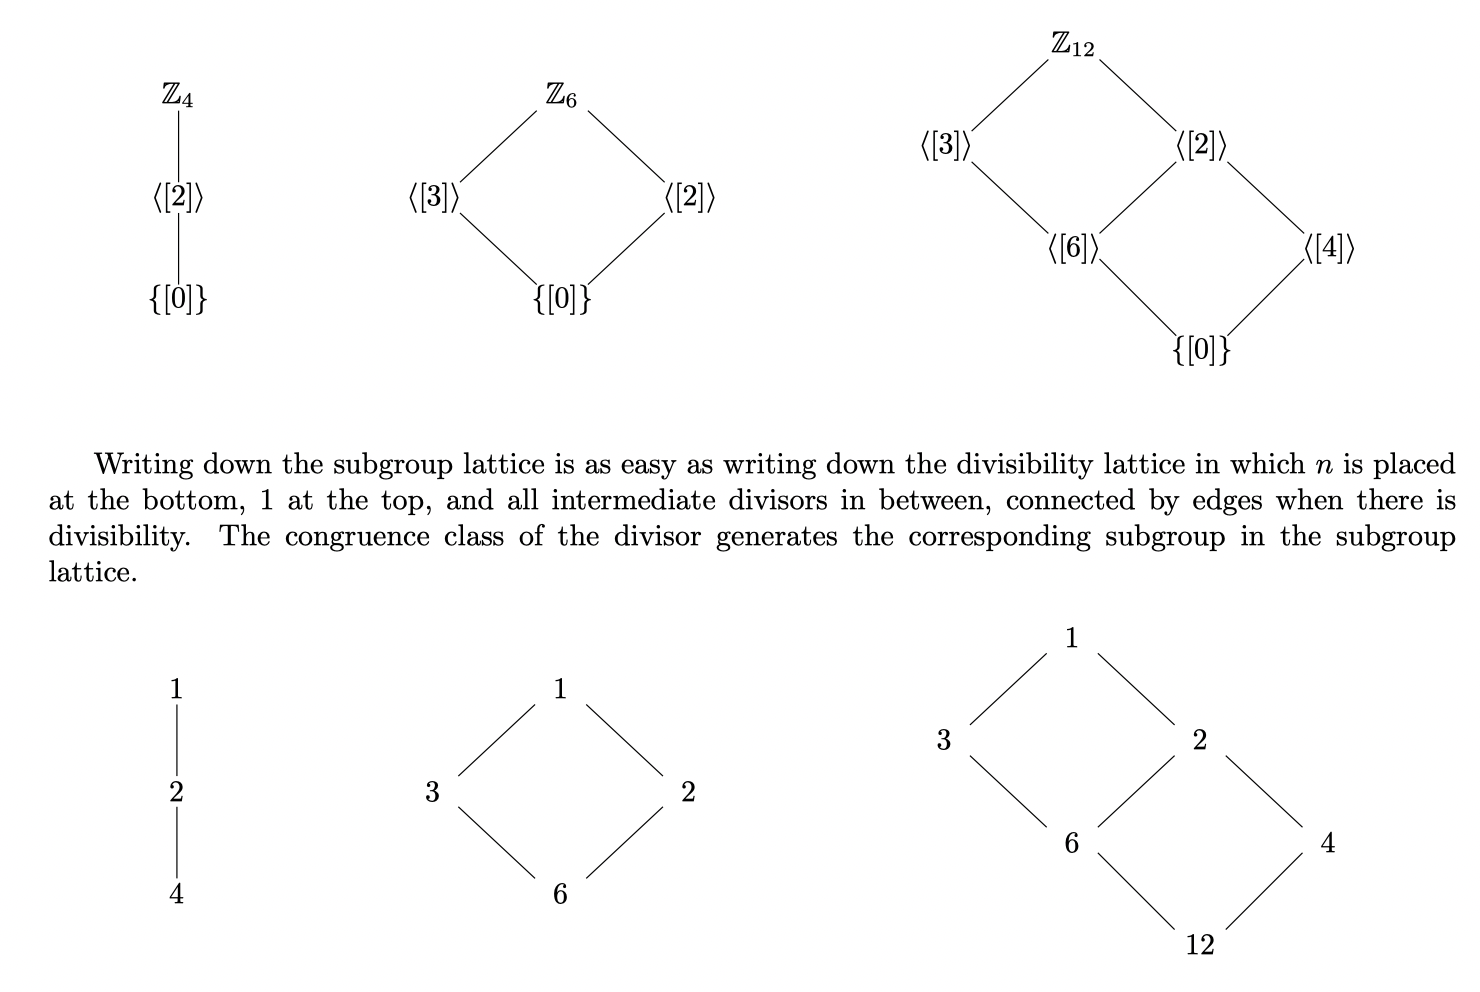
\includegraphics[scale=0.6]{lec1301.png}
    \caption{}
    \label{}
\end{figure}\end{center}









\section{Ring $(R,+,\cdot)$: $+$ is associative, commutative, identity, inverse $\in R$; $\cdot$ is associative, distributes over $+$}
\begin{definition}
    A ring is a nonempty set with two operations, called addition and multiplication, $(R,+,\cdot)$ such that
\end{definition}
(1): $(R,+)$ is an ablian group: i.e. $+$ is associatve and commucative. $0,-a\in R$\\
(2): $\cdot$ is associative.\\
(3): $\cdot$ distributes over $+$: $\forall a,b,c\in R$, $a\cdot(b+c)=a\cdot b+a\cdot c$ and $(b+c)\cdot a=b\cdot a+c\cdot a$
\subsection{Commutative ring: ring's $\cdot$ is commutative}
If "$\cdot$" is commutative, we call $(R, +, \cdot)$ a commutative ring.
\subsection{Ring with 1: exists multiplication identity $1\in R$}
If there exists an element $1\in R\backslash \{0\}$ such that $a1=1a=a,\ \forall a\in R$,then we say that $R$ is a ring with 1.

\subsection{Field $\mathbb{F}$ is a commutative ring with 1; $\mathbb{F}[x]$ is also a commutative ring with 1}
Field $(\mathbb{F}, +, \cdot)$ (close, associative, commutative, distributive(M over A), identity $\&$ inverse(M,A))\\
Proposition 2.3.2: Polynomial ring (close, associative, commutative, distributive(M over A), identity(M,A), inverse(only A))

\subsection{$S\subset R$: Subring (closed under $+$ and $\cdot$; addictive inverse $-a\in S$)}
\subsubsection{Proposition 2.6.27: $(S,+,\cdot)$ is a ring}
\begin{proposition}[Proposition 2.6.27]
    If $S\subset R$ is a subring, then $+,\cdot$ make $S$ into a ring.
\end{proposition}

































































































\begin{thebibliography}{1}      \bibitem{Long2015Fully}  Christopher J Leininger  \newblock Introduction to Abstract Algebra
    (Draft)  2017.
\end{thebibliography}


\end{document}
\bibliography{reference}
\bibliographystyle{unsrt}